\section{Visual Evidence Atlas}

The main paper already contains the compact figures needed for the submission narrative. This
atlas adds new explanatory plates and diagrams for reviewers who want to inspect the diagnostic
logic visually. The plates cover predicate anatomy, failure storyboards, package accounting,
robot-link ownership, and provenance flow. Every final figure in this section is a supplement-only
asset under \texttt{figures/generated/supplement/}; none is a copy of a main-paper figure.

\subsection{Failure Storyboards}

Failure labels can look terse in a table. The storyboard format separates the initial state,
terminal state, measured symptom, and emitted label. This makes it easier to see that a failure is
not an omitted baseline or dependency gap: the package was generated, mapped, simulated, and then
rejected by a named probe.

\begin{figure}[!ht]
\centering
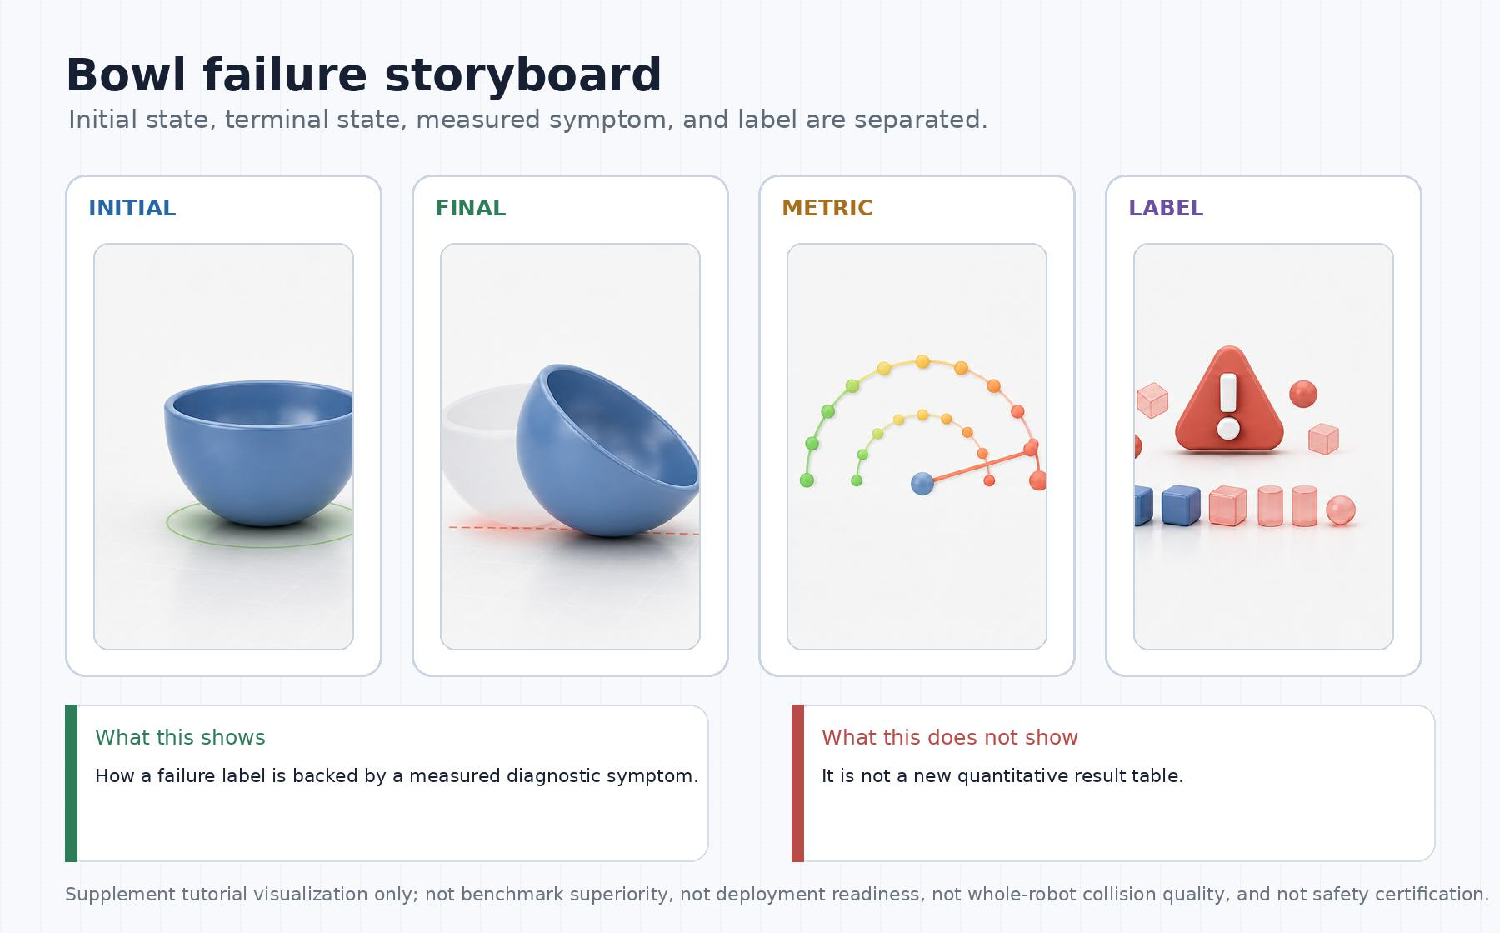
\includegraphics[width=0.84\textwidth]{figures/generated/supplement/supplement_failure_storyboard_bowl.pdf}
\caption{Supplement-only bowl failure storyboard. The storyboard format separates the simulated
states, measured symptom, and emitted label.}
\label{fig:supp-failure-storyboard-bowl}
\end{figure}
\FloatBarrier

\paragraph{What this shows.}
Figure~\ref{fig:supp-failure-storyboard-bowl} shows how a diagnostic failure label is anchored in
state measurements. The value of the storyboard is not photorealism; it is the separation of cause,
measurement, and label.

\paragraph{What this does not show.}
The storyboard is not a new quantitative result and should not be read as a broad statement about
all bowls, all V-HACD settings, or all primitive packages.
\FloatBarrier

\begin{figure}[!ht]
\centering
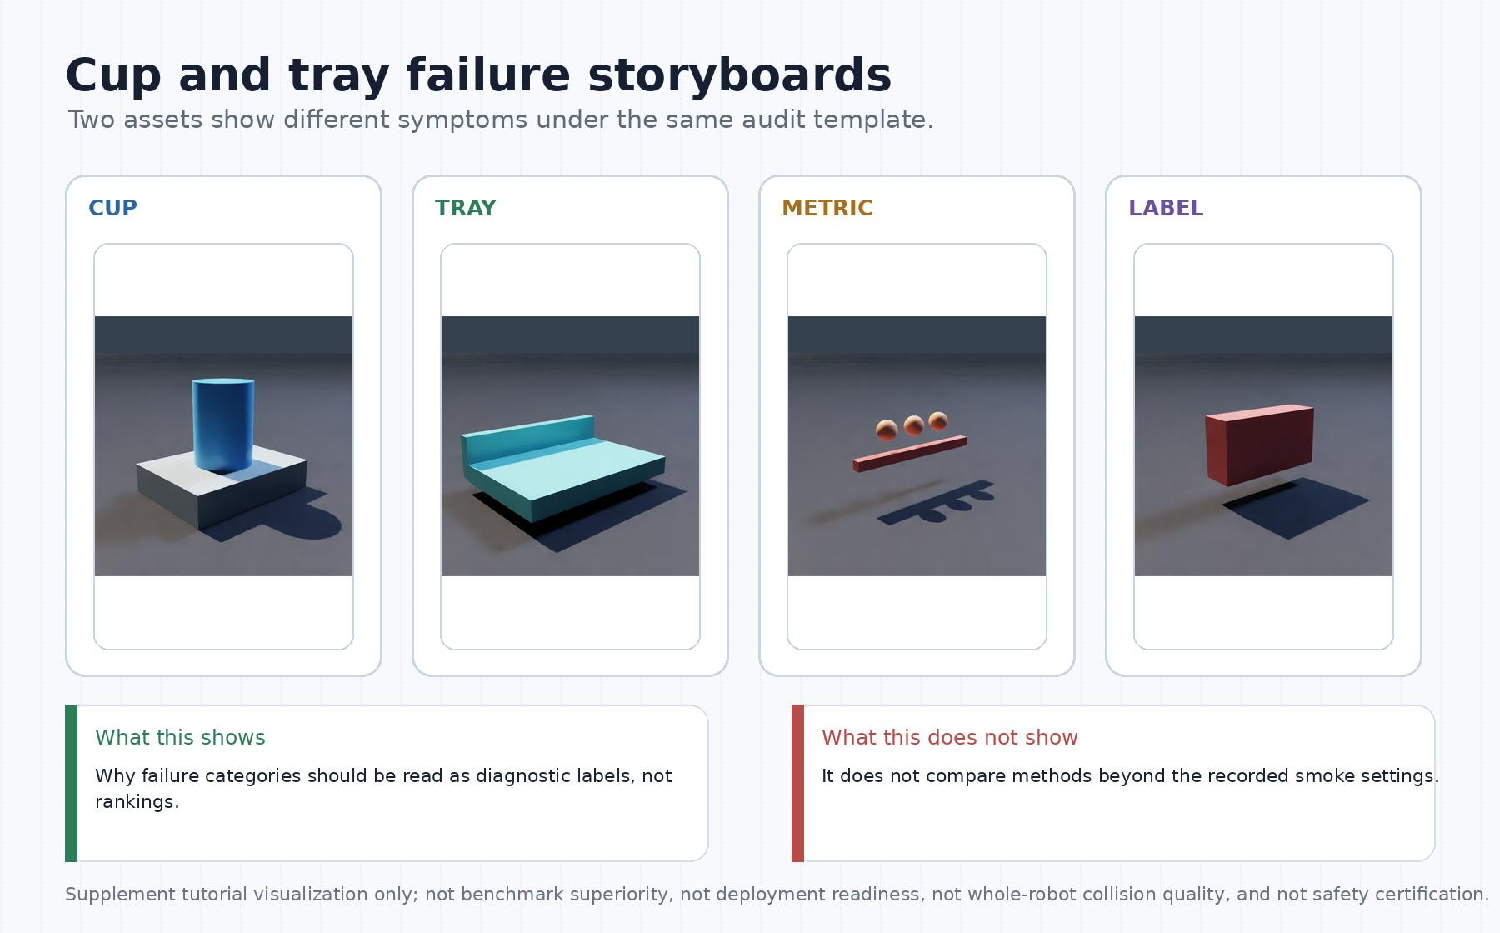
\includegraphics[width=0.84\textwidth]{figures/generated/supplement/supplement_failure_storyboard_cup_tray.pdf}
\caption{Supplement-only cup and tray failure storyboards. Two assets are shown with the same
diagnostic-template logic but different measured symptoms.}
\label{fig:supp-failure-storyboard-cup-tray}
\end{figure}
\FloatBarrier

\paragraph{What this shows.}
Figure~\ref{fig:supp-failure-storyboard-cup-tray} shows why failure labels should be kept
probe-specific. Different assets can fail different clauses even when they pass through the same
candidate-lane and diagnostic-checker interface.

\paragraph{What this does not show.}
The plate does not rank candidate generators and does not claim that one failure mode dominates a
larger benchmark.
\FloatBarrier

\subsection{Rigid and Robot Visual Reading Rules}

The atlas uses restrained, source-separated visual styles on purpose. The figures are not meant to
replace source assets, raw renders, task logs, or dated records. They are meant to make the audit
path legible: source package, generated package, diagnostic scene, measured symptom, and claim
boundary.

\begin{table}[t]
\centering
\footnotesize
\caption{Visual-reading guide for supplement figures. This table explains how to interpret the
new atlas plates without expanding the evidence boundary.}
\label{tab:supp-visual-reading}
\setlength{\tabcolsep}{3pt}
\renewcommand{\arraystretch}{1.08}
\begin{tabular}{@{}>{\raggedright\arraybackslash}p{0.22\linewidth}@{\hspace{0.035\linewidth}}>{\raggedright\arraybackslash}p{0.42\linewidth}@{\hspace{0.035\linewidth}}>{\raggedright\arraybackslash}p{0.22\linewidth}@{}}
\toprule
Visual element & Intended reading & Do not infer \\
\midrule
Colored boxes & generated package components or link-owned bodies & geometric optimality \\
Arrows and gauges & measured diagnostic terms or state transitions & full dynamics coverage \\
Failure cards & emitted probe labels from recorded symptoms & broad baseline ranking \\
Franka link sketches & ownership and attachment semantics & manipulation success \\
Provenance boxes & reproducible paper artifact chain & external submission content \\
\bottomrule
\end{tabular}
\end{table}

\paragraph{Atlas limitation.}
The final plates are organized for readability, not for new evidence. They help reviewers follow
the audit path, while runtime evidence remains in dated records and manifests.
